\documentclass[12pt,a4paper,titlepage]{report}
\usepackage{polski}
\usepackage[utf8]{inputenc}
\usepackage{amsmath}
\usepackage{amsfonts}
\usepackage{amssymb}
\usepackage{graphicx}
\usepackage{listings}
\usepackage{enumerate}
%hiperłącza
\usepackage{hyperref}
\hypersetup{
    colorlinks,
    citecolor=black,
    filecolor=black,
    linkcolor=black,
    urlcolor=black
}
%XML
\usepackage{color}
\definecolor{dkgreen}{rgb}{0,0.6,0}
\definecolor{gray}{rgb}{0.5,0.5,0.5}
\definecolor{mauve}{rgb}{0.58,0,0.82}
\definecolor{gray}{rgb}{0.4,0.4,0.4}
\definecolor{darkblue}{rgb}{0.0,0.0,0.6}
\definecolor{lightblue}{rgb}{0.0,0.0,0.9}
\definecolor{cyan}{rgb}{0.0,0.6,0.6}
\definecolor{darkred}{rgb}{0.6,0.0,0.0}


\lstset{
  	basicstyle=\ttfamily\footnotesize,
  	columns=fullflexible,
  	showstringspaces=false,
  	numbers=left,                   % where to put the line-numbers
  	numberstyle=\tiny\color{gray},  % the style that is used for the line-numbers
  	stepnumber=1,
  	numbersep=5pt,                  % how far the line-numbers are from the code
  	backgroundcolor=\color{white},      % choose the background color. You must add \usepackage{color}
  	showspaces=false,               % show spaces adding particular underscores
  	showstringspaces=false,         % underline spaces within strings
  	showtabs=false,                 % show tabs within strings adding particular underscores
  	frame=none,    
  	xleftmargin=10px,              % adds a frame around the code
  	rulecolor=\color{black},        % if not set, the frame-color may be changed on line-breaks within not-black text (e.g. commens (green 	here))
  	tabsize=2,                      % sets default tabsize to 2 spaces
  	captionpos=b,                   % sets the caption-position to bottom
  	breaklines=true,                % sets automatic line breaking
  	breakatwhitespace=false,        % sets if automatic breaks should only happen at whitespace
  	%title=\lstname,                   % show the filename of files included with \lstinputlisting;
 		                              % also try caption instead of title  
  	commentstyle=\color{gray}\upshape
}
 \lstdefinelanguage{XML}{
  	morestring=[s][\color{mauve}]{"}{"},
  	morestring=[s][\color{black}]{>}{<},
  	morecomment=[s]{<?}{?>},
  	morecomment=[s][\color{dkgreen}]{<!--}{-->},
  	stringstyle=\color{black},
  	identifierstyle=\color{lightblue},
  	keywordstyle=\color{red},
  	morekeywords={xmlns,xsi,noNamespaceSchemaLocation,type,id,x,y,source,target,version,tool,transRef,roleRef,objective,eventually},
}


\author{Katarzyna Węgiełek \\ Paweł Własiuk \\ Kamil Sienkiewicz\\ Marcin Wardziński}
\title{\textbf{Computational Cluster}}
\linespread{1.125}

\begin{document}
	\maketitle
	\tableofcontents

	\chapter{Wstęp}
	Tematem projektu jest stworzenie dokumentacji dla klastra obliczeniowego. Zadaniem projektowanego przez nas systemu będzie prowadzenie obliczeń rozproszonych. Klaster będzie umożliwiał rozwiązywanie skomplikowanych problemów, wykorzystujących algorytmy o dużej złożoności czasowej, w szczególności rzędu o($2^n$). Jego najważniejszą rolą będzie odpowiednie rozdzielenie zadań pomiędzy różne elementy systemu tak, aby jak najbardziej optymalnie wykorzystywać moc obliczeniową komputerów, z których się składa. Istotne jest również zminimalizowanie ryzyka utraty danych w przypadku awarii któregoś z komponentów.
	
	\section{Elementy klastra obliczeniowego}
	\textbf{Task manager} - dzieli zadanie na podproblemy i oblicza rozwiązanie końcowe na podstawie rozwiązań częściowych\\\\
\textbf{Computational node} - rozwiązuje pojedynczy podproblem i odsyła do jego rozwiązanie częściowe do communications server'a\\\\
\textbf{Communications server} - przesyła podproblemy i rozwiązania częściowe między task manager'ami a computational node'ami oraz wysyła rozwiązanie zadania do computational client'a\\\\
\textbf{Computational client} - wysyła problem do communications server'a i oczekuje na otrzymanie rozwiązania\\\\
\textbf{Task solver} - moduł używany przez computational node do rozwiązania podproblemu oraz przez task manager do podzielenia zadania i znalezienia ostatecznego rozwiązania na podstawie wyników częściowych\\
	
	\chapter{Opis działania systemu}
	Proces rozwiązywania zadania rozpoczyna się od wprowadzenia przez użytkownika danych wejściowych dla problemu. Robi to za pośrednictwem \emph{computational client'a}. Jest to jedyny element klastra, z którym użytkownik ma bezpośredni kontakt. \emph{Computational client} przetwarza wprowadzone informacje na komunikat i wysyła do \emph{communications server'a} w formie pliku XML.\\
	Następnie zadanie trafia do kolejki zgłoszonych problemów. Jeśli istnieje w danej chwili w klastrze wolny \emph{task manager}, który potrafi obsłużyć zadanie tego typu, to \emph{communications server} wysyła do niego otrzymane dane wejściowe. \emph{Task manager} dzieli problem na mniejsze części - podproblemy, przeznaczone do rozwiązania przez pojedyncze \emph{computational node'y} i odsyła je do \emph{server'a}. To czy \emph{task manager} może podzielić dany problem zależy od tego, czy posiada \emph{task solver}, zajmujący się poszukiwaną klasą problemów.\\
	\emph{Communications server} wysyła odebrane podproblemy kolejno do wolnych \emph{computational node'ów}, które są w stanie je rozwiązać (zawierają odpowiedni \emph{task solver}). \emph{Node'y} prowadzą obliczenia równolegle, a następnie wysyłają uzyskane wyniki do \emph{server'a}. \emph{Communications server} przesyła rozwiązania częściowe do \emph{task managera}, który oblicza na ich podstawie ostateczny wynik. \emph{Task manager} zaczyna scalanie dopiero po otrzymaniu wszystkich rozwiązań częściowych. Gdy uzyska końcowe rozwiązanie, wysyła je do \emph{server'a}. Trafia ono do kolejki zadań oczekujących na odebranie wyników. Kiedy \emph{computational client} wyśle do \emph{server'a} żądanie pobrania rozwiązania, \emph{server} odsyła mu odpowiednie dane.\\
Podczas całego procesu główny \emph{communications server} synchronizuje trzymane przez siebie dane z \emph{server'em backup'owym}, aby w razie awarii nie stracić części rozwiązań i zgłoszonych zadań. Jeśli \emph{server} główny ulegnie uszkodzeniu i komunikacja z nim będzie niemożliwa, pozostałe komponenty nie przerwą swojej normalnej pracy i zaczną wymieniać komunikaty z \emph{server'em backup'owym}.

	\section{Diagram aktywności dla rozwiązania pojedynczego problemu}
	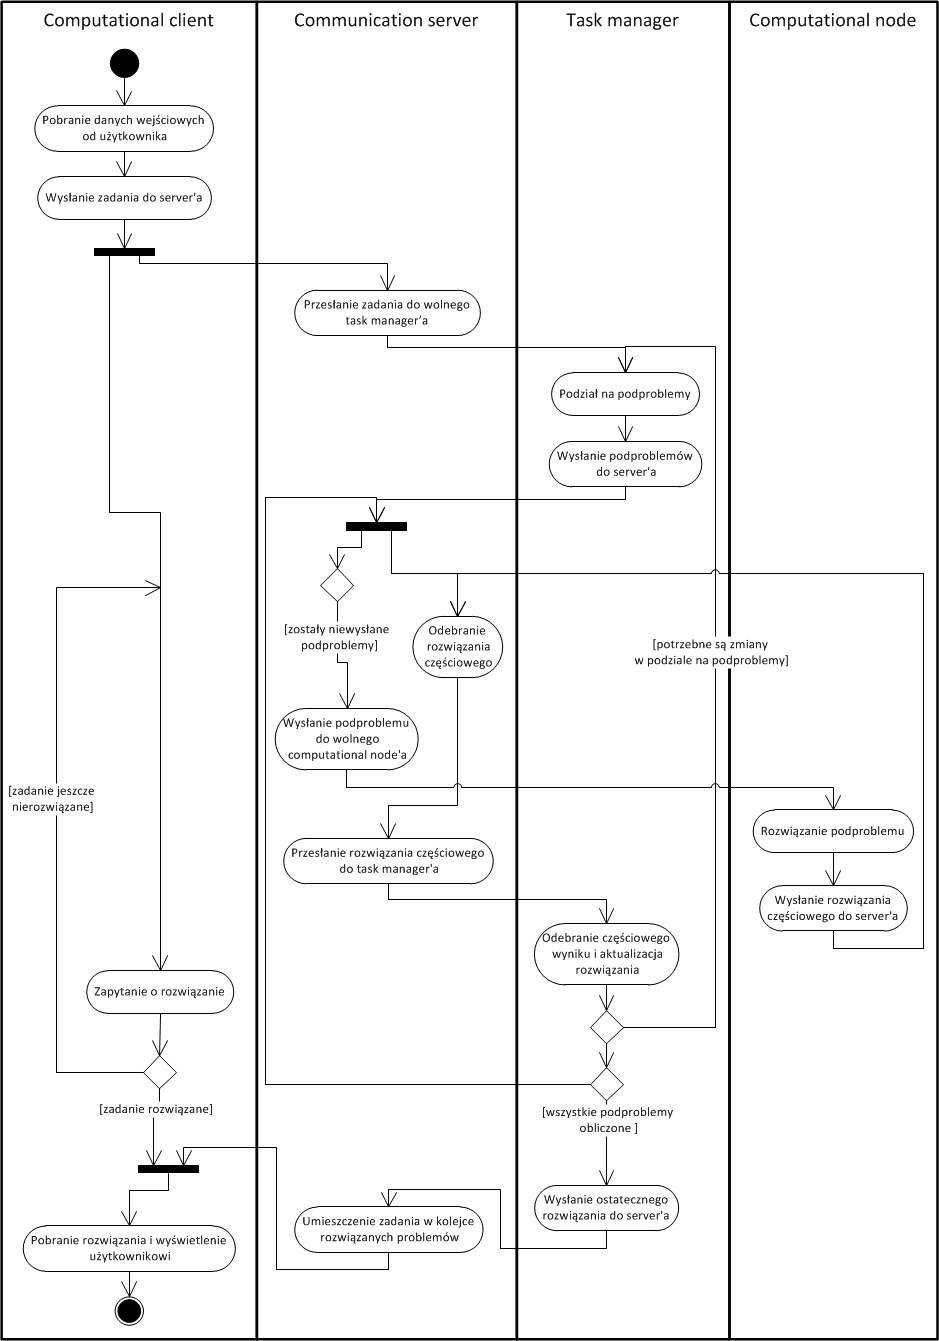
\includegraphics[width=\textwidth]{img/activityDiagram.png}
	
	\section{Diagramy przypadków użycia}	
	\subsection{Diagram przypadków użycia dla użytkownika}
	Główną rolą użytkownika jest zdefiniowanie problemu do rozwiązania przez klaster obliczeniowy. Wprowadza on dane wejściowe dla zadania za pośrednictwem \emph{computational client'a}. Gdy obliczenia zostają zakończone, użytkownik pobiera z \emph{communications server'a} rozwiązanie (również za pośrednictwem aplikacji klienckiej). Użytkownik w dowolnym momencie może sprawdzić, czy prace nad jego problemem zostały już zakończone. Na jego żądanie \emph{communications server} wysyła do \emph{computational client'a} listę wszystkich zadań, które zostały już rozwiązane. Jeśli interesujący go problem znajduje się na liście, użytkownik wskazuje identyfikator zadania i pobiera rozwiązanie.\\
	
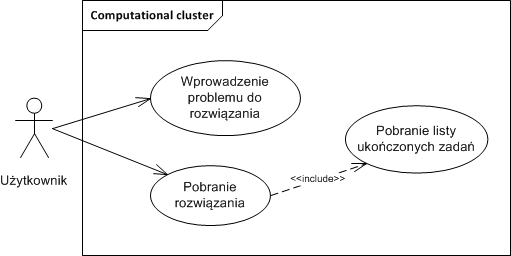
\includegraphics[width=\textwidth]{img/usecaseUser.png}	
	
	\subsection{Diagram przypadków użycia dla administratora}
	Administrator ma za zadanie skonfigurować wszystkie elementy klastra. Najpierw uruchamia \emph{primery communications server} oraz \emph{backup server}. Następnie dołącza do sieci pozostałe komponenty - \emph{task manager'y}, \emph{computational node'y} i \emph{computational client'ów}. Aby umożliwić komunikację pomiędzy elementami systemu, administrator musi zapisać w pliku konfiguracyjnym przyłączanego elementu adresy IP obu serwerów. Żeby \emph{task manager} i \emph{computational node} mogły brać udział w rozwiązywaniu problemu, muszą mieć zainstalowany przynajmniej jeden \emph{task solver}. Zatem przy dołączaniu ich do klastra administrator powinien zainstalować odpowiednią wtyczkę.\\
Nowe komponenty mogą być dodawane zarówno przy tworzeniu klastra, jak i już podczas jego działania. Administrator może również w każdym momencie wgrać do \emph{task manager'a} lub \emph{computational node'a} kolejne \emph{task solver'y}, odpowiadające nowym klasom problemów. Zwiększy się w ten sposób ilość typów zadań, jakie klaster jest w stanie rozwiązać.\\

	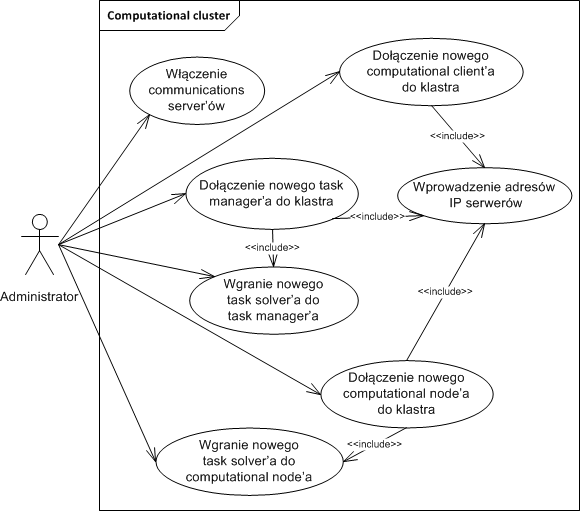
\includegraphics[width=\textwidth]{img/usecaseAdmin.png}	
	
		
	\chapter{TaskSolver}
		\section{Interfejs}	
	\begin{figure}[h]
		\centering
		\caption{Interfejs pluginu}
		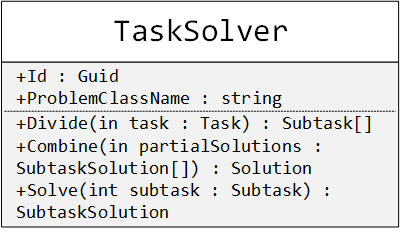
\includegraphics[width=0.6\textwidth]{img/taskSolverInterface.png}
	\end{figure}
	
	Komponenty systemu odpowiedzialne za wykonywanie obliczeń będą korzystały z interfejsu zaprezentowanego powyżej.
	Klasa obsługiwana przez system musi implementować 3 metody konieczne do rozwiązania zadania:
	\begin{itemize}
		\item \verb+Divide()+ - metoda, która jako parametr przyjmuje \textit{zadanie}. Jej głównym zadaniem
		 jest podzielenie problemu
		na mniejsze łatwiejsze do rozwiązania podproblemy.
		\item \verb+Combine()+ - metoda, która w parametrze przyjmuje kolekcję częściowych rozwiązań. Jej zadaniem
		jest scalenie rozwiązań częściowych w jedno ostateczne rozwiązanie.
		\item \verb+Solve()+ - metoda jako parametr przyjmuje podzadanie, które powstało w wyniku działania metody \verb+Divide+. 
		Efektem działania tej metody jest rozwiązanie problemu.
	\end{itemize}		
	
	Plugin powinien również udostępniać dwa pola umożliwiające zidentyfikowanie obiektów tej samej klasy
	w różnych częściach systemu:
	\begin{itemize}
		\item \verb+Id+ - unikalne pole typu \verb+Guid+. System nie przewiduje istnienia dwóch różnych klas,
		rozwiązujących różne zadania identyfikujących się identycznym id. Taka sytuacja mogłaby doprowadzić system do błędu.
		\item \verb+ProblemClassName+ - pole typu \verb+string+ zawierające informację zrozumiałą dla użytkownika
		o typie problemu rozwiązywalnego przez daną klasę.
	\end{itemize}		

	Rozwiązanie problemu powinno przebiegać w poniżej podany sposób:
		\begin{enumerate}[(1)]
			\item zadanie zostaje podzielone na podzadania,
			\item każde z podzadań zostaje rozwiązane,
			\item wszystkie rozwiązania częściowe zostają przekazane jako parametr metody scalającej rozwiązania
			w wyniku czego otrzymujemy końcowe rozwiązanie naszego problemu.
		\end{enumerate}
	 \section{Instalacja Pluginów}
	Komponenty klastra odpowiedzialne za obliczenia tj. \textit{Task Manager} i \textit{Computational Node} przy każdym odpytaniu serwera o listę klas problemów, które mogą rozwiązać będą przeszukiwać folder \verb+TaskSolvers+ znajdujący się w katalogu z aplikacją, w celu poszukiwania bibliotek z klasami implementującymi interfejs \verb+TaskSolver+. Gdy komponentowi zostanie zlecone zadanie, ten wykorzystując mechanizm refleksji wyszuka w katalogu odpowiednią klasę i stworzy jej instancję. Obiekt ten  umożliwi realizacją zleconego zadania.\\
	 Instalacja nowych pluginów w komponentach systemu będzie sprowadzała się wyłącznie do wklejenie biblioteki z klasą implementującą interfejs \verb+TaskSolver+ do wyżej wymienionego katalogu.	
	
	
	\chapter{Computational client}
	Zadaniem \emph{computational client'a} jest pobranie danych wejściowych od użytkownika i wysłanie do \emph{communications server'a} zlecenia rozwiązania podanego problemu. Gdy obliczenia zostaną zakończone, klient odbiera od serwera rozwiązanie zadania i prezentuje otrzymane wyniki użytkownikowi. Aby sprawdzić czy konkretne zadanie zostało już obliczone, \emph{computational client} pobiera z \emph{server'a} listę wszystkich ukończonych zleceń.\\
	
	\section{Zlecenie rozwiązania problemu}
	Użytkownik zleca klastrowi obliczeniowemu rozwiązanie zadania za pośrednictwem \emph{computational client'a}. Określa typ problemu, jaki ma zostać obliczony oraz wprowadza dane wejściowe. \emph{Computational client} zapisuje odebrane dane w formacie XML, a następnie wysyła komunikat do \emph{communications server'a}. Aplikacja kliencka nawiązuje połączenie z \emph{server'em} używając adresu IP, zapisanego w pliku konfiguracyjnym. Po odebraniu zlecenia od \emph{client'a}, \emph{server} umieszcza nowe zadanie w kolejce problemów odpowiedniego typu oczekujących na rozwiązanie. Zadanie znajduje się w kolejce dopóki któryś z \emph{task manager'ów} potrafiących obsłużyć problem tej klasy nie zakończy wcześniejszych obliczeń i nie będzie mógł się nim zająć.\\
	
	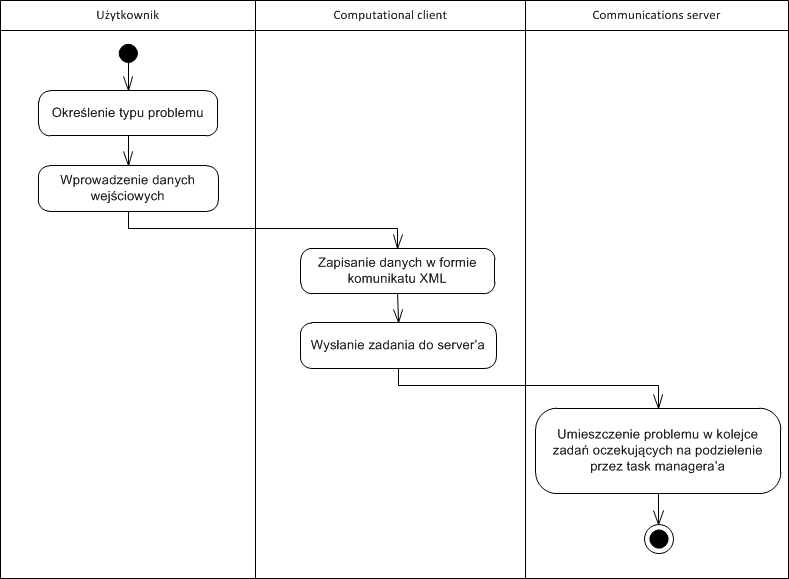
\includegraphics[width=\textwidth]{img/activityDiagramClient1.png}
	
	\section{Pobranie rozwiązania}	
	Po otrzymaniu rozwiązania problemu od \emph{task manager'a}, \emph{communications server} umieszcza je na liście ukończonych zadań. Gdy użytkownik chce zobaczyć rozwiązanie swojego problemu, \emph{computational client} wysyła do \emph{server'a} zapytanie i otrzymuje listę wszystkich wyników. Jeśli poszukiwane zadanie znajduje się na tej liście to znaczy, że \emph{computational cluster} skończył już jego obliczanie. \emph{Client} pobiera wtedy z \emph{server'a} rozwiązanie i wyświetla je użytkownikowi. Jeżeli obliczenia nie zostały jeszcze zakończone, użytkownik dostaje komunikat, że nadal trwa rozwiązywanie zadania.
	
	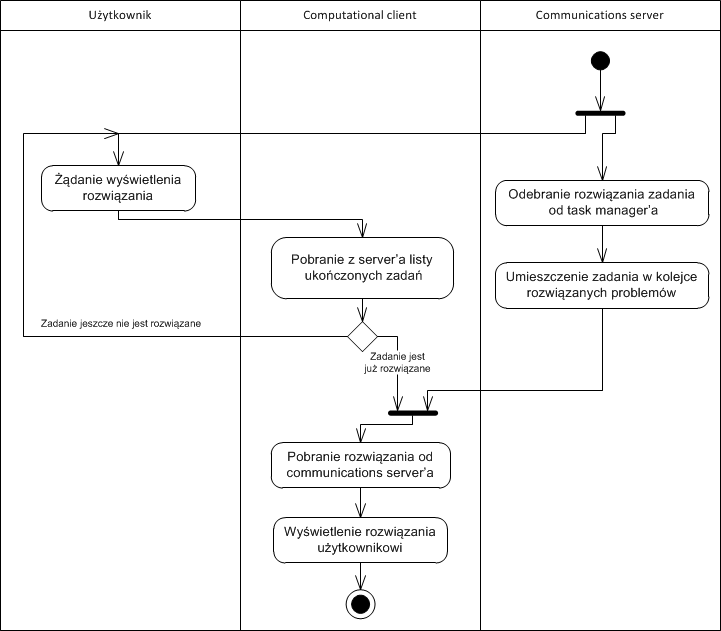
\includegraphics[width=\textwidth]{img/activityDiagramClient2.png}
	
\chapter{Communication server}
		Communication server sprawuje najważniejszą rolę w działaniu całego systemu. Zajmuje się
		przyjmowaniem zadań oraz przydzielaniem zasobów potrzebnych do ich rozwiązania,
		dba o poprawne i bezpieczne przechowywanie wyników i innych obiektów komunikacyjnych.
		Pełni rolę swojego rodzaju pośrednika w komunikacji między innymi elementami klastra.
		
		Communication server ze względu na swoje znaczenie ma możliwość podłączenia dodatkowego
		communication server'a uruchomienia w trybie \textit{backup}, z którym będzie
		prowadzona dodatkowa synchronizacja danych, w celu bezproblemowego działania
		w przypadku utraty jednego z nich.
		
		Dla zwiększenia czytelności przedstawiony zostanie tryb normalny, różnice w trybie
		backup zostaną uwidocznione w osobnym podrozdziale.
		
		
	\section{Cykl życia serwera}
		Communication server zaraz po uruchomieniu sprawdza poprawność własnej konfiguracji,
		istnienia niezbędnych zależności (bazy danych). Gdy wszystko przebiegnie pomyślnie
		tworzy dwa wątki - nasłuchujący oraz operacyjny.
		
		Wątek nasłuchujący zajmuje się oczekiwaniem i obsługiwaniem wstępnym nadchodzących 
		komunikatów z innych komponentów klastra obliczeniowego. Konkretne zachowanie zależne
		jest od rodzaju komunikatu, jeżeli otrzymujemy zapytanie o parametry serwera
		odpowiedź finalna jest udzielana od razu, ale jeśli jest to zlecenie podzadania,
		poprawne przyjęcie jest sygnalizowane dopiero po synchronizacji z drugim communication server'em,
		jeśli taki jest ustawiony i dostępny.
		
		Wątek operacyjny zaś, nieustannie (gdy ma taką możliwość) dba o redundancję danych wymieniając 
		się danymi z innym communication server'em będącym w trybie \textit{backup} oraz rozsyła komunikaty 
		przydzielając poszczególne zadania,	ze względu na zachowanie ciągłości synchronizacji ilość 
		przydzielonych zadań w jednym cyklu jest dobierana eksperymentalnie i całkowicie konfigurowalna.
		Co jakiś czas wątek ten sprawdza również obecność wszystkich komponentów i aktualizuje ich listy
		obsługiwanych wtyczek. 
		
		Ogólny diagram aktywności communication server'a można znaleźć na rysunku 
		~\ref{CommunicationServerGeneralActivity}.
		
		\begin{figure}
			\centering
			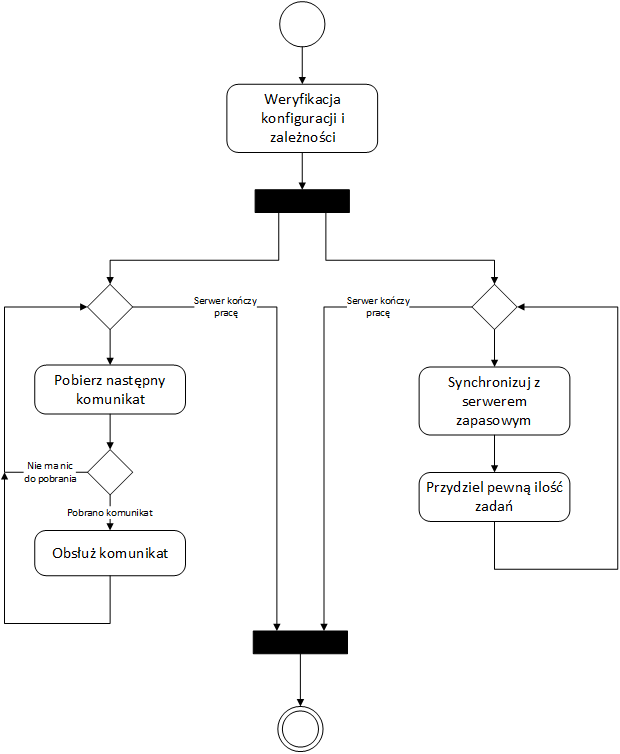
\includegraphics[width=\textwidth]{img/CommunicationServer-General.png}
			\caption{Ogólny diagram aktywności communication server'a}
			\label{CommunicationServerGeneralActivity}
		\end{figure}
		
	\section{Cykl życia zadania}
	
		Dla każdego zadania możemy wyodrębnić kilka jego głównych stanów. Nowo zlecone zadanie
		trafia nieprzetworzone do odpowiedniej kolejki, oczekując na przesłanie do task manager'a
		i podzielenie na łatwiejsze do rozwiązania podproblemy. Po podzieleniu, zadanie czeka na rozwiązanie
		wygenerowanych podzadań, a po ich otrzymaniu wygenerowane jest rozwiązanie, które oczekuje potem na
		pobranie przez użytkownika; lub zgłaszane są dodatkowe podzadania potrzebne do wygenerowania poprawnego
		wyniku.
		
		\begin{figure}[h]
			\centering
			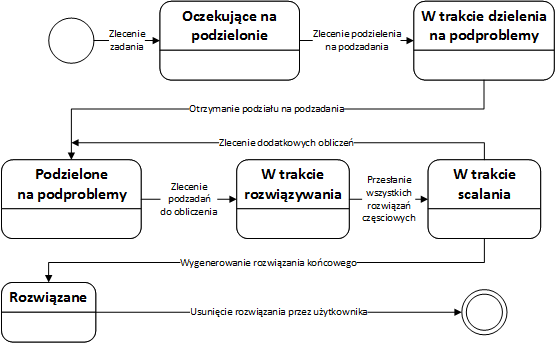
\includegraphics[width=\textwidth]{img/state/Task.png}
			\caption{Diagram stanów zadania}
		\end{figure}
		
	\section{Przydzielanie zadań}
		W celu optymalnego przechowywania zleconych przez użytkownika zadań opracowaliśmy
		strukturę ich przechowywania w której główny podział stanowi rodzaj problemu
		(TSP, DVRP itp.), a jego w obrębie znajdują się osobne listy FIFO dla nowo zgłoszonych problemów,
		podproblemów do rozwiązania oraz podproblemów do scalenia. Rodzaj problemu dla przyspieszenia obliczeń
		przechowywuje także informacje o menadżerach zadań i węzłach obliczeniowych, które potrafią
		go obsłużyć. 
		
		Communication server w momencie wyboru zadania filtruje rodzaje problemów w poszukiwaniu takich,
		które są mają oczekujące zadania oraz są rozwiązywalne, czyli posiadają do dyspozycji wolny task manager 
		oraz mają zlecone jakieś zadanie. Spośród tych rodzajów wybieramy zadanie zlecone najwcześniej, by zachować
		oczekiwaną kolejność zajmowania się z zadaniami.
		
		Przy przydzielaniu podzadań dla poszczególnych computational node'ów postępujemy analogicznie.
		
		Rozwiązania podzadań odsyłamy do task manager'a w celu scalenia po otrzymaniu ich wszystkich. Menadżer
		po analizie odpowiedzi może zdecydować o wygenerowaniu rozwiązania końcowego lub zlecić podzadania dodatkowe
		i odłożyć końcową odpowiedź na termin późniejszy. 
		
		\begin{figure}[h]
			\centering
			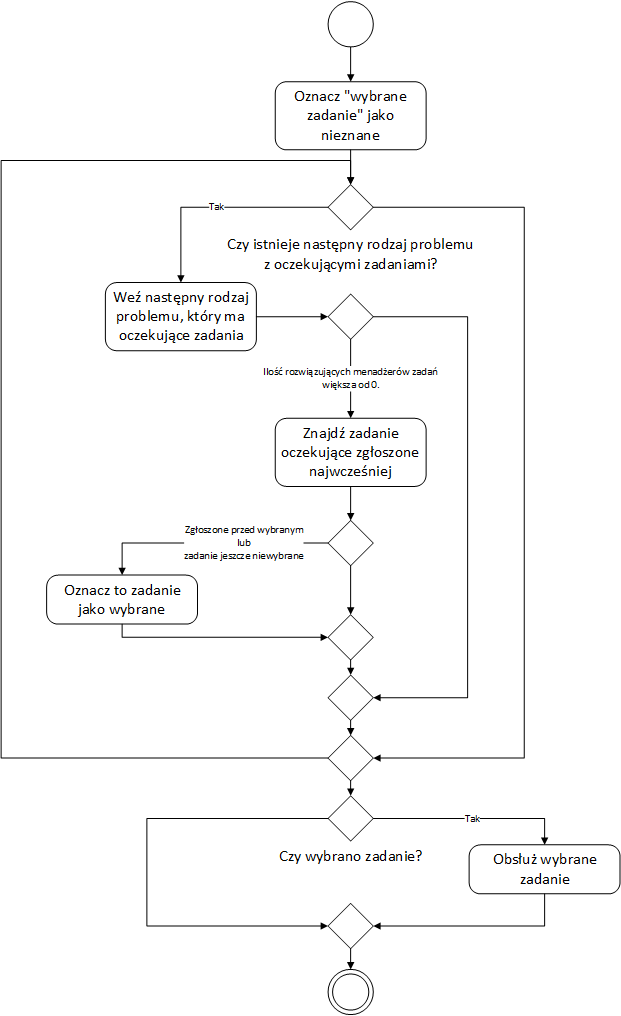
\includegraphics[width=\textwidth]{img/CommunicationServer-SelectTask.png}
			\caption{Wybór zadania przez communication server}
		\end{figure}
		
		Nie należy zapominać również o zadaniach które zostały zlecone, ale z jakichś powodów
		nie zostały wykonane w oczekiwanym czasie. Takie zadania wracają do kolejki i czekają na
		ponowne przydzielenie.
		
	\section{Tryb backup}
		Serwer w trybie backup zachowuje się bardzo podobnie do serwera w trybie normalnym.
		Najistotniejszą różnicą jest to, że stara się on być jedynie nośnikiem danych
		i nie wykonywać żadnych operacji na dostępnych zasobach. W przypadku próby zlecenia
		mu zadania podczas gdy nie jest on jedynym serwerem przekierowuje je do głównego 
		communication server'a.	Jeżeli zaś communication server nie odpowiada, przejmuje jego obowiązki.
		W momencie przywrócenia sprawności serwera głównego, synchronizują się one w normalnym
		trybie, a serwer główny staje się w pełni operacyjny.
		
	\section{Synchronizacja między serwerami}
		Obiekty w czasie stworzenia i zapisania do jednej z baz danych oznaczane są jako obiekty
		do synchronizacji i są wymieniane między serwerami w następnym cyklu w formie wiadomości
		synchronizacyjnej. Podobnie dzieje się z zmodyfikowanymi obiektami (modyfikowane
		mogą być jedynie pola z datą przydzielenia pracy i informacją o zleceniobiorcy).
		Po otrzymaniu potwierdzenia odebrania są oznaczone jako zsynchronizowane. Jeśli
		potwierdzenie nie zostanie otrzymane, wykonywana jest retransmisja po odpowiednim
		czasie oczekiwania.
	
	\chapter{Task manager}
		Task Manager do podziału zadania wykorzystuje Task Solvera, który obsługuje odpowiedni dla klasy zadania plugin. Na tym etapie nie są obliczane konkretne drogi (w przypadku DVRP), a tylko ich identyfikatory. Task Manager, znając liczbę Node'ów, zamawia w Task Solverze podział zadania na odpowiednią liczbę części. Każdy Node dostaje potem polecenie obliczenia opcji między jednym a drugim identyfikatorem, pewien przedział problemów. Obliczanie konkretnych dróg nie miałoby sensu, oznaczałoby wykonanie przez Task Managera pracy Node'a.
		
		Częściowe rozwiązania są przechowywane przez Task Managera. Łączenie zadania polega na wyborze najbardziej optymalnego rozwiązania. Odbywa się to znowu przez Task Solvera, wykorzystując metodę klasy problemu, która porównuje rozwiązania.
	
	\chapter{Communicational node}
		Zadanie communicational node'a sprowadza się do uruchomienia w Task Solverze czasochłonnej metody obliczającej w pętli wydajność wszystkich rozwiązań zawartych między podanymi identyfikatorami. W trakcie obliczeń, Node informuje Serwer co określony czas, że jest zajęty. Po zakończeniu wyniki zostają wysłane przez serwer do Task Managera.
	
	 
	%komunikacja + schemy
	\chapter{Komunikacja}
		\section{Nawiązywania połączenia}
	Uruchomienie całego systemu rozpoczyna się od uruchomienia \textit{Communications Server'a}. Od tej chwili komponenty systemu tj. 
	\textit{Computational node'y}	i \textit{Task Managery} mogą zgłaszać swoją obecność w klastrze. Każdy z komponentów systemu 
	posiada w swoim pliku konfiguracyjnym (w węzłach \verb+MainServerAddress+ i \verb+BackupServerAddress+) \textbf{adres IP} i
	 \textbf{port} \textit{Communications Server'a} oraz serwera zapasowego. Zaraz po uruchomieniu każdy komponent
	zgłasza swoją obecność do głównego serwera. Po trzech nieudanych próbach nawiązania połączenia następuje
	wysłanie identycznej informacji do serwera backup'owego. Każdy z komponentów w takiej wiadomości informuje o swoim rodzaju podaje
	IP i port na którym	działa. Na tej podstawie serwer będzie komunikował się z tymi elementami systemu.\\
	
		 \lstinputlisting[caption=\footnotesize{Wiadomość wysyłana przez komponent włączający się do systemu},language=XML,firstline=1,lastline=6]{examples.xml} 
		
	Parametr \verb+ComponentType+ informuje o rodzaju komponentu systemu. Wartości, które może przyjąć ten parametr to:
	\begin{itemize}
		\item \verb+TaskManager+ - w przypadku gdy wiadomość pochodzi od \textit{Task Manager'a},
		\item \verb+ComputationalNode+ - gdy wiadomość pochodzi od \textit{Computational Node'a}
	\end{itemize} 

	Zadaniem \textit{Communications Server'a} jest utrzymywanie listy aktywnych komponentów systemu, oraz przechowywanie informacji
	na temat klas problemów, które dane komponenty obsługują. W tym celu serwer regularnie, co pewien określony czas
	będzie odpytywał wszystkie swoje komponenty prosząc o listę klas problemów możliwych do rozwiązania. W przypadku gdy takiej
	odpowiedzi nie otrzyma uznaje komponent za wyłączony i usuwa jego dane z pamięci. W przypadku otrzymania odpowiedzi na
	żądanie, serwer na podstawie otrzymanych danych uzupełnia/aktualizuje informacje o rozwiązywalnych problemach
	przez komponenty.\\
	
		\lstinputlisting[caption=\footnotesize{Odpowiedź komponentu na żądanie serwera},language=XML,firstline=8,lastline=14]{examples.xml} 

	W wiadomości, dla każdego typu problemu zostają przekazane dwie informacje:
	\begin{itemize}
		\item \verb+problemClassName+ - nazwa problemu,
		\item \verb+problemClassId+ - guid problemu, który w jednoznaczny sposób identyfikuje typ problemu.	
	\end{itemize} 		
		
	\begin{figure}[h]
		\centering
		\caption{Uzyskiwanie połączenia przez komponent systemu}
		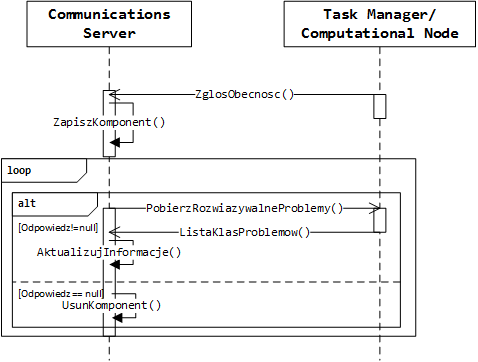
\includegraphics[width=0.8\textwidth]{img/communication/connecting.png}
	\end{figure}
	
	\section{Lista rozwiązywalnych problemów}
	Proces rozwiązywania zadania przez \textit{Computational Cluster} rozpoczyna się na poziomie \textit{Computational client'a}. Przed
	wysłaniem problemu do rozwiązania, aplikacja kliencka musi pobrać z serwera informację na temat klas problemów
	rozwiązywalnych w danej chwili przez \textit{Computational Cluster} (wynika ona z obecnie dostępnych \textit{Menadżerów zadań} i
	\textit{Computational Node'ów}). Aplikacja kliencka odpytuje \textit{serwer komunikacyjny} o potrzebne informacje. 
	Serwer w odpowiedzi na to żądanie odsyła wiadomość, w której zawarte są informacje o wszystkich typach problemów
	rozwiązywalnych przez klaster. Informacje zostają przetworzone i przedstawione użytkownikowi. Wiadomość przesłana do 
	\textit{Computational Clienta} jest identyczna z tą, którą serwer otrzymuje od pozostałych komponentów systemu.
	
	\begin{figure}[h]
		\centering
		\caption{Diagram sekwencji pobierania informacji z serwera przez \textit{Computational Client'a}}
		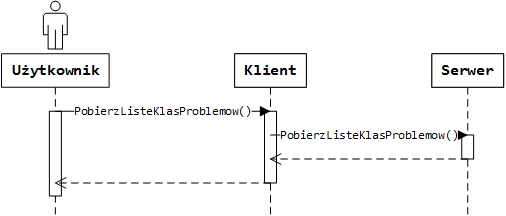
\includegraphics[width=0.9\textwidth]{img/communication/problemclass.png}
	\end{figure}	
	
	\section{Rozwiązywanie zadania}
	
	Po wykonaniu czynności opisanych w poprzednim rozdziale, użytkownik może zlecić zadanie \textit{klastrowi obliczeniowemu}
    \textit{Computational Client} wysyła do serwera wiadomość z informacją o typie rozwiązywanego problemu i dane wejściowe zadania.\\
    
    \lstinputlisting[caption=\footnotesize{Zlecenie rozwiązania zadania przez \textit{Computational Client'a}},language=XML,firstline=16,lastline=20]{examples.xml}
    
     Wiadomość zawiera 2 parametry konieczne do stworzenia i rozwiązania zadania:
    \begin{itemize}
    	\item \verb+problemClassId+ - identyfikator klasy problemu, umożliwiający zidentyfikowanie, które części systemu są w stanie rozwiązać dany problem
    	\item \verb+Data+ - parametry typu \verb+String+ zawierający dane wejściowe dla danego typu problemu. Dane te przedstawione są w formacie XML odpowiednim dla danego typu problemu.  
    \end{itemize}
    
    Serwer po otrzymaniu wiadomości generuje specjalny identyfikator, który przypisuje do zadania. Będzie on wykorzystany do 
    identyfikacji poszczególnych podzadań oraz umożliwi klientowi zidentyfikowanie zleconego zadania.\\
    
    \lstinputlisting[caption=\footnotesize{Informacja z tokenem zwracana do aplikacji klienckiej},language=XML,firstline=22,lastline=25]{examples.xml}
    
    Taki token zostaje również odesłany do aplikacji klienckiej, która zapisze go w swoim pliku konfiguracyjnym. Poniżej przykład prezentujący odpowiedni wpis:
    
    \begin{lstlisting}[language=XML,numbers=none]
    <TaskList>
    	<Task taskname="customTaskName1" taskToken="ee28fec2-6361-4a58-aaf1-b9ff0f509743"/>
    	<Task taskname="customTaskName2" taskToken="4fbcbba1-014e-4643-b60f-f7888a95bb54"/>
    </TaskList>
    \end{lstlisting}
    Węzeł \verb+Task+ odpowiada jednemu zleconemu zadaniu przez użytkownika. Każdy taki węzeł posiada dwa atrybuty:
	
	\begin{itemize}
		\item \verb+taskToken+ - to identyfikator zadania nadany przez klaster obliczeniowy, dzięki niemu użytkownik będzie miał możliwość pobrania rozwiązania zadania,
		\item \verb+taskname+ - nazwa zadania nadana przez użytkownika, która umożliwi mu zidentyfikowanie zadania, nazwa obecna wyłącznie na poziomie aplikacji klienckiej.
	\end{itemize}	    
      
	
	\begin{figure}[h]
		\centering
		\caption{Diagram sekwencji pobierania informacji z serwera przez \textit{Computational Client'a}}
		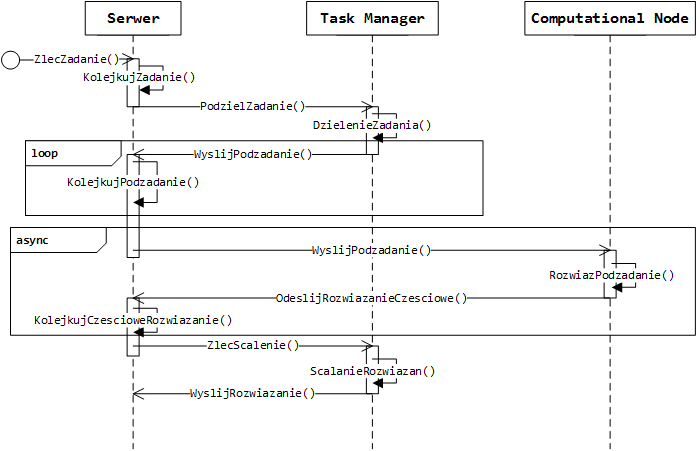
\includegraphics[width=\textwidth]{img/communication/computation.png}
	\end{figure}    
    
    
    \textit{Computational Cluster} wykonuje ciąg czynności koniecznych do otrzymania rozwiązania, tzn:
	\begin{enumerate}[(1)]
		\item przesłanie polecenia podziału zadania od \textit{serwera} do \textit{Task Manager'a} - wiadomość w formacie otrzymanym od \textit{Computational Client'a},
		\item podział zadania i odesłanie stworzonych podproblemów prowadzących do otrzymania rozwiązania. \textit{Task Manager} dokonuje podziału zadania, każdemu z nich przydzielając unikalny identyfikator. Wiadomość zwrotna zawiera informacje o 
		typie rozwiązywalnego problemu, identyfikatora zadania, identyfikatora podzadania, oraz danych wejściowych potrzebnych do rozwiązania zadania.
		
		\lstinputlisting[caption=\footnotesize{Zlecenie podzadania},language=XML,firstline=36,lastline=42]{examples.xml}
		
		\item przesłanie każdego z podzadań do \textit{węzłów obliczeniowych}
		\item przeprowadzenie obliczeń i odesłanie częściowych rozwiązań do \textit{serwera}. Odsyłana wiadomość zawiera informacje o 
		typie rozwiązywalnego podproblemu, identyfikatorze zadania, identyfikatorze podzadania oraz rozwiązaniu częściowym problemu.
		\item przesłanie częsciowych rozwiązań do \textit{Task Managera} w celu stworzenia rozwiązania. Przesłanie wiadomości wcześniej zebranych od \textit{Computational Node'ów}.
		\item odesłanie pełnego rozwiązania zadania do \textit{serwera} w identycznym formacie jak te, które serwer odsyła do \textit{Computational Clienta}
	\end{enumerate}

	Zadanie przesłane do podziału przez \textit{Communications server} jest w formacie otrzymanym od \textit{Computational Client'a}    
    
    \section{Odczytanie rozwiązania}	
	Proces odczytywania rozwiązania zadania rozpoczyna się od załadowania listy zadań zleconych przez daną aplikację z pliku konfiguracyjnego do którego wcześniej zostały wpisane identyfikatory poszczególnych zadań. Użytkownik wybiera zadanie którego rozwiązanie
	chce pobrać. Aplikacja odpytuje serwer o rozwiązanie, w wyniku czego otrzymuje informację na jego temat. Wiadomość, którą wysyła aplikacja kliencka w węźle \verb+TaskId+ zawiera identyfikator zadania którego rozwiązania oczekujemy.\\

	 \lstinputlisting[caption=\footnotesize{Rozwiązanie zadania},language=XML,firstline=28,lastline=34]{examples.xml}

	\begin{figure}[h]
		\centering
		\caption{Diagram sekwencji pobierania informacji z serwera przez aplikację kliencką}
		 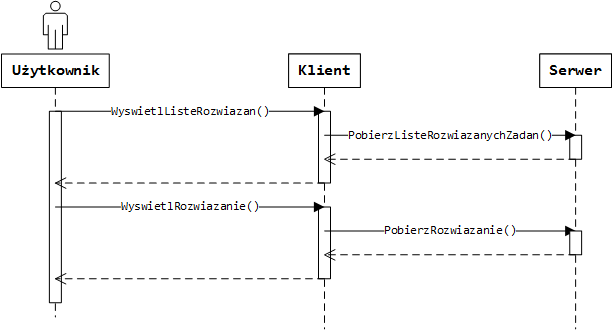
\includegraphics[width=\textwidth]{img/communication/getresult.png}
	\end{figure} 	
	
	Wiadomość otrzymana od serwera składa się z 4 węzłów:
	\begin{itemize}
		\item \verb+problemClassId+ - identyfikator klasy problemów, której dotyczy zadanie. Informacja potrzebna do odpowiedniego wyboru 
		pluginu, który odpowiednio sparsuje i przedstawi wyniki użytkownikowi.
		\item \verb+TaskId+ - identyfikator zadania
		\item \verb+Status+ - dwie możliwe wartości to \verb+Done+ - jeżeli zadanie zostało ukończone oraz \verb+InProgress+ - jeżeli rozwiązywanie zadania nadal trwa.
		\item \verb+Data+ - w przypadku gdy status przyjmuję wartość \verb+Done+ pole zawiera rozwiązanie zadania w postaci XML,
		w przeciwnym przypadku wartość jest pusta
	\end{itemize}
	
	\section{Schema}
		\subsection{Uzyskiwanie połączenia przez komponenty}	
			\lstinputlisting[language=XML]{schema/connectionMessageSchema.xsd}
		\subsection{Lista rozwiązywalnych problemów przez klaster obliczeniowy}
			\lstinputlisting[language=XML]{schema/SolvableProblemListMessage.xsd}
		\subsection{Zlecenie rozwiązania zadania}
			\lstinputlisting[language=XML]{schema/TaskOrderMessage.xsd}
		\subsection{Token wysyłany do aplikacji klienckiej}
			\lstinputlisting[language=XML]{schema/TaskTokenMessage.xsd}
		\subsection{Żądanie o przesłanie rozwiązania zadania}
			\lstinputlisting[language=XML]{schema/TaskResultRequestMessage.xsd}
		\subsection{Rozwiązanie Zadania}
			\lstinputlisting[language=XML]{schema/TaskResultMessage.xsd}
		\subsection{Zlecenie rozwiązania podzadania}
			\lstinputlisting[language=XML]{schema/SubtaskOrderMessage.xsd}
		\subsection{Przesłanie rozwiązania podzadania}
			\lstinputlisting[language=XML]{schema/SubtaskResultMessage.xsd}
			
\chapter{Przykład algorytmu}
		W tym miejscu działanie klastra zostanie omówione na przykładzie DVRP. Problem marszrutyzacji można rozpatrywać jako rozwinięcie problemu komiwojażera i chińskiego listonosza. Dostawca np. pizzy ma za zadanie rozwieść towar do klientów. Z punktu początkowego może wyruszać wiele pojazdów. Na podstawie wag krawędzi optymalizowany jest czas, odległość albo cena. Dynamic w nazwie problemu oznacza, że część klientów będzie dostępna dopiero o konkretnej godzinie.
		
		Klient wysyła do Serwera komunikacyjnego prośbę o rozwiązanie DVRP, listę krawędzi z wagami oraz liczbę dostawców. Serwer przekazuje problem do wolnego Menedżera zadań, który potrafi dzielić ten problem. Menedżer pyta serwer o liczbę dostępnych węzłów z Task solverem obsługującym DVRP.
		
		Menedżer zadań, za pomocą Task Solvera używa metody klasy problemu, by wyznaczyć zakres identyfikatorów dróg dla poszczególnych Nodeów. Klasa problemu DVRP zawiera ściśle ustalony porządek możliwych podziałów na drogi i dostawców. Dlatego też Node będzie w stanie zrozumieć instrukcję, że ma obliczyć przykładowo możliwości między 5, a 19. W głównej pętli programu zostaną wstawione odpowiednie wartości.
		
		Węzeł za pomocą Task Solvera używa metody klasy problemu DVRP, by wyznaczyć przyznane mu trasy oraz ich koszty. Informuje też serwer, że jest w trakcie obliczeń. Gdy je zakończy, przesyła przez Serwer do Menadżera wszystkie pośrednie wyniki. Menadżer pod koniec obliczeń wybiera najbardziej optymalną trasę (najmniej kilometrów, najniższy koszt  itp.), znowu za pomocą metody scalającej z klasy DVRP, odpalanej przez Task Solvera. Przesyła ją przez serwer do klienta.
		
\end{document}
